\documentclass[a4paper]{article}
\usepackage{amssymb,amsmath,amsthm,amsfonts}
\usepackage{multicol,multirow}
\usepackage{calc}
\usepackage{ifthen}
\usepackage{graphicx}
\usepackage{float}
\usepackage[landscape]{geometry}
\usepackage[colorlinks=true,citecolor=blue,linkcolor=blue]{hyperref}


\ifthenelse{\lengthtest { \paperwidth = 11in}}
    { \geometry{top=.5in,left=.5in,right=.5in,bottom=.5in} }
	{\ifthenelse{ \lengthtest{ \paperwidth = 297mm}}
		{\geometry{top=1cm,left=1cm,right=1cm,bottom=1cm} }
		{\geometry{top=1cm,left=1cm,right=1cm,bottom=1cm} }
	}

\pagestyle{empty}
\makeatletter
\renewcommand{\section}{\@startsection{section}{1}{0mm}%
                                {-1ex plus -.5ex minus -.2ex}%
                                {0.5ex plus .2ex}%x
                                {\normalfont\large\bfseries}}
\renewcommand{\subsection}{\@startsection{subsection}{2}{0mm}%
                                {-1explus -.5ex minus -.2ex}%
                                {0.5ex plus .2ex}%
                                {\normalfont\normalsize\bfseries}}
\renewcommand{\subsubsection}{\@startsection{subsubsection}{3}{0mm}%
                                {-1ex plus -.5ex minus -.2ex}%
                                {1ex plus .2ex}%
                                {\normalfont\small\bfseries}}
\makeatother
\setcounter{secnumdepth}{0}
\setlength{\parindent}{0pt}
\setlength{\parskip}{0pt plus 0.5ex}
% -----------------------------------------------------------------------

\title{Performance Analysis CheatSheet}

\begin{document}

\raggedright
\footnotesize

\begin{center}
     \Large{\textbf{Performance Analysis Formula Sheet }} \\
\end{center}
\begin{multicols*}{3}
\setlength{\premulticols}{1pt}
\setlength{\postmulticols}{1pt}
\setlength{\multicolsep}{1pt}
\setlength{\columnsep}{2pt}

\section{Probability Review}
\subsection{Identities}
\begin{flalign*}
    & P(A \cap B) = P(A)P(B)  \\
    & P(A|B) = \frac{P(A \cap B)}{P(B)}
    & P(A) = P(A|B)P(B) + P(A|\bar B)P(\bar B) \\
    & f(x) = \frac{dF(x)}{dx}, \int_{-\infty}^\infty f(x)=1
    & P(a < X < b) = \int_a^{b} f(x) dx  \\ 
    & F(y) = \int_{-\infty}^y f(x)dx   
    & P(X < x) = F(X)  \\
    & \mathbb{E}[X^n] =  \int_{-\infty}^\infty x^n f(x) dx
    & Var(X) = \mathbb{E}[X^2] - \mathbb{E}[X]^2 
\end{flalign*}

\subsection{Uniform Distribution: $X \sim uniform(a,b)$}
\begin{flalign*}
    & f(x)= 
        \begin{cases}
            \frac{1}{b-a},  & \text{if } a < x < b\\
            0,              & \text{otherwise}
        \end{cases}&  \tag{pdf} \\
    & F(x)= 
        \begin{cases}
            0,              & \text{if } x < a  \\
            \frac{x-a}{b-a},  & \text{if } a \leq x \leq b\\
            1,              & \text{if } x > b
        \end{cases} \tag{cdf} \\
    & \mathbb{E}[X] = \frac{a+b}{2} 
    & Var[X] = \frac{(b-a)^2}{12} \\
\end{flalign*}

\subsection{Exponential Distribution:  $ X \sim exp(\lambda)$}
\begin{flalign*}
    & f(x)= \lambda e ^{-\lambda x} \tag{pdf} \\
    & F(x)= 1 - \lambda e ^{-\lambda x} \tag{cdf} \\
    & \mathbb{E}[X] = \frac{1}{\lambda}
    & Var[X] = \frac{1}{\lambda^2}  \\
    & P(X > s+t | X>s) = P(X >t) 
    & \text{[Memoryless]} \\
\end{flalign*}

\subsection{Poisson Distribution: $ X \sim pois(\lambda)$}
\begin{flalign*}
    & P(N(t) = n) = \frac{(\lambda t)^t}{n!} e^{-\lambda t} 
    & \text{[pmf]} \\
    & \mathbb{E}[X] = Var(X) \\
\end{flalign*}


\subsection{Poisson Process}
\begin{flalign*}
    & N(0) = 0 \\
    & f(x)= \lambda e ^{-\lambda x} 
    & \text{[Arrival See Time Average]} \\
    & P(X > s+t | X>s) = P(X >t) 
    & \text{[Memoryless]} \\
    &  \lambda = \sum _{i=1}^{n}\lambda _{i}, Y = \left(\sum _{i=1}^{n}X_{i}\right)\sim \operatorname {pois}(\lambda)
    & \text{[Merge Poisson Processes]} \\
    & X \sim pois(\lambda), X = [X_1, X_2] \\
    & \implies X_{1,2} \sim pois(\frac{\lambda}{2})
    & \text{[Split Poisson Processes]}
\end{flalign*}

\columnbreak

\section{Performance Analysis}
\subsection{Identities}
\begin{flalign*}
    & A_i(t)  \text{  [Number of arrivals]}
    & \lambda_i(t) = \frac{A_i(t)}{t} \text{ [Arrival Rate]} \\
    & C_i(t) \text{ [Completions] } 
    & X_i(t) = \frac{C_i(t)}{t} \text{  [Throughput]} \\
    & B_i(t)  \text{  [Busy time]} 
    & \rho_i(t) = \frac{B_i(t)}{t} \text{  [Utilization]} \\
    & S_i(t) = \frac{B_i(t)}{C_i(t)}
    \text{  [Avg process time]}
    & S_i(t) = \mathbb{E}[S]  \\
    & D_i  \text{ [Processing time of cycle]} 
    & \mathbb{E}[D_i] = \mathbb{E}[S_i]\mathbb{E}[Vi] \\
    & V_i(t)  \text{  [Visits to device]} 
    & V_{user} = V_0 = 1 \\ 
    & \lim_{t \to \infty} \frac{A_i(t)}{t} = \lim_{t \to \infty} \frac{C_i(t)}{t} 
    & \lambda_i = X_i \text{ [Steady state]} \\
    & N(t) = A(t) - C(t) 
    & \text{  [Number of jobs in system]} \\
    & R(t) \approx \int_0^t \frac{A(s) - C(s)}{A(t)}ds
    & \text{  [Avg response time]} \\
    & \bar N(t) \approx \int_0^t \frac{A(s)-C(s)}{t} ds
    & \text{  [Avg number of jobs in system]} \\
    & \bar N(t) = \frac{R(t)A(t)}{t} \\
    & Z  
    & \text{ [Think time] } \\
    & \mathbb{E}[N] = N, \lambda = X, R = R + Z 
    & \text{[Closed System]}
\end{flalign*}
 
\subsection{Operation Laws}
\begin{flalign*}
    & \rho_i = \mathbb{E}[S_i] X_i = \frac{\lambda_i}{\rho_i}
    & \text{[Utilization Law]} \\
    & \rho_i = \mathbb{E}[S_i]\mathbb{E}[Vi]X =  \mathbb{E}[D_i] X
    & \text{[Bottleneck Law]} \\
    & X_i = \mathbb{E}[V_i]X 
    & \text{[Forced Flow Law]}\\
    & \mathbb{E}[N] = \lambda \mathbb{E}[R]
    & \text{[Little's Law]} \\ 
    & \mathbb{E}[N_i] = \lambda_i \mathbb{E}[R_i] \\
    & \mathbb{E}[R] = \frac{N}{X} - \mathbb{E}[Z] 
    & \text{[Closed System Response Time Law] } \\
\end{flalign*}


\subsection{Bottleneck Analysis}
\begin{flalign*}
    & D_{max} \text{  [Bottleneck Device]}
    & D = \sum D_i \\
    & \mathbb{E}[R] \geq D 
    & X = \frac{\rho_{max}}{D_{max}} \\
    & \mathbb{E}[R] \geq max(D, ND_{max} - \mathbb{E}[Z])
    & X \leq  min(\frac{1}{D_{max}}, \frac{N}{D+\mathbb{E}[Z]}) \\
    & N^* = \frac{D + \mathbb{E}[Z]}{D_{max}} 
    & \implies \text{optimal } X \text{ and } \mathbb{E}[R] \\
\end{flalign*}

\columnbreak

\section{Queuing Models}
(Arrivals / Service Times / Number of servers / Room in system)
 
\subsection{M/M/1}
\begin{flalign*}
    & \rho = \lambda/\mu 
    & \mu > \lambda \text{  [Stability condition]}\\
    & \pi_0 =  1 - \frac{\lambda}{\mu} = 1 - \rho
    & \pi_i = \pi_0 (\frac{\lambda}{\mu})^i  = (1-\rho)\rho^i \\
    & \mathbb{E}[N] = \frac{\lambda}{\mu - \lambda}  = \frac{\rho}{1-\rho}
    & \mathbb{E}[N_Q] = \mathbb{E}[N] - \rho \\
    & \mathbb{E}[R] = \frac{1}{\mu - \lambda} 
    & \mathbb{E}[R_Q] = \frac{1}{\mu - \lambda} - \frac{1}{\mu} \\
\end{flalign*}

\begin{figure}[H]
    \vspace{-1cm}
    \centering
    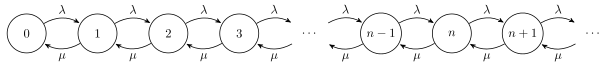
\includegraphics[scale=0.35]{MM1-queue.png}
\end{figure}

\subsection{M/M/c}
\begin{flalign*}
    & \rho = \frac{\lambda}{c\mu} 
    & c\mu > \lambda \text{  [Stability condition]} \\
    & \pi_0 =  (\frac{\lambda}{\mu})^c \frac{1}{1 - \rho} 
    % TODO Fix from notes:
    & \pi_i = 
        \begin{cases}
            \frac{\lambda^i}{i!\mu^i} \pi_0,  & \text{if } i < c \\
            \frac{\lambda^i}{c!\mu^ic^{i-c}} \pi_0,              & \text{if } i \geq c 
        \end{cases}&  \\ 
    & \mathbb{E}[N] = \lambda \mathbb{E}[R] 
    & \mathbb{E}[N_Q] = \lambda \mathbb{E}[R_Q] \\
    & \mathbb{E}[R] = \mathbb{E}[R_Q] + \mathbb{E}[S] = \mathbb{E}[R_Q] +  \frac{1}{\mu} \\
    & \mathbb{E}[R_Q] = \frac{(\frac{\lambda}{\mu})^c \mu}{(c-1)! (c\mu - \lambda)^2} \\
    & P(\text{job is queued}) = \sum_{i=0}^\infty \pi = \frac{1}{c!}(\frac{\lambda}{\mu})^c \frac{1}{1-\rho} \pi_0
    & \text{[Erlang C Formula]}
\end{flalign*}

\begin{figure}[H]
    \vspace{-0.25cm}
    \centering
    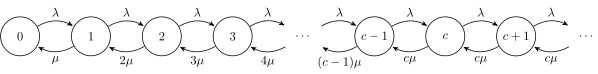
\includegraphics[scale=0.35]{MMC-queue.png}
\end{figure}

\vspace{-0.25cm}
\subsection{M/M/$\infty$}
\begin{flalign*}
    & \rho = \lambda/\mu 
    & \mu > \lambda \text{ [Always Stable]}\\
    & \pi_0 =  e^{-\frac{\lambda}{\mu}} = e^{-\rho}
    & \pi_i = \frac{(\lambda/\mu)^i}{i!} e^{-\frac{\lambda}{\mu}} = \frac{\rho^i}{i!} e^{-\rho} \\
    & \mathbb{E}[N] = \frac{\lambda}{\mu} = \rho 
    & \mathbb{E}[N_Q] = 0 \\
    & \mathbb{E}[R] = \frac{1}{\mu} = \mathbb{E}[S] 
    & \mathbb{E}[R_Q] =  0 \\
\end{flalign*}

\begin{figure}[H]
    \vspace{-1cm}
    \centering
    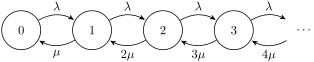
\includegraphics[scale=0.4]{MMinfinity-queue.png}
\end{figure}


\subsection{Birth-Death Process}
CTMC where state transitions increase or decrease by a constant factor.
%TODO check notes for pi_0
\[
    \pi_0 = \frac{1}{1 + \sum_{k=1}^{\infty} \prod_{i=1}^k \frac {\lambda _{i-1}}{\mu_i} }
\]
\[
    \pi_i = \frac{\prod_{j=0}^{i-1} \lambda_j}{ \prod_{j=1}^{i} \mu_j}\pi_0
\]

\subsection{Threshold System}
$T>0$, Arrival rate $s$, processing rate $s$. If $r > s, N \to 0$. If $s >r, N \to \infty$.  
\[
    \pi_0 = \frac{1}{1 - \frac{r}{s}} (\frac{s}{r})^T-1
\]
\[
    \pi_i = 
        \begin{cases}
            (\frac{s}{r})^i \pi_0,  & \text{if } i < T \\
            (\frac{s}{r})^{i-T} (\frac{r}{s})^2 \pi_0, & \text{if } i \geq T
        \end{cases}
\]


\section{Misc}
\begin{itemize}
    \item 
     $\sum_{i=0}^\infty \alpha^i = \frac{1}{1-\alpha}, |\alpha| < 1 $.
    
    \item
    $h = \frac{f}{g} \implies h' = \frac{f'g -fg'}{g^2}$
    
    \item
    Blocking system structure $\implies X_1 = X_2 = ... = X_n$
    
    \item
    Max system utilization $\implies$ only bottleneck utilization is 100\%
    
    \item
    Want to minimize $\mathbb{E}[R]$ and maximize $X$.
    
    \item
    Operation Laws work regardless of distributions of random variables

    \item
    exponential distributions are a very good assumption for modeling arrivals, but only moderately good for modelling processing times
\end{itemize}

% \section{Strategy/Notable Questions}





% \section{Performance operational analysis}
% \subsection{Operational Laws}
% \begin{align*}
%     \langle H \rangle(\lambda) &= 
%     \frac{\langle \psi(x,\lambda)|H|\psi(x,\lambda) \rangle}{\langle \psi(x,\lambda)|\psi(x,\lambda) \rangle} \\
%     \langle H \rangle(\lambda) &\geq E_{.g.s} \\
%     \frac{d}{d\lambda} \langle H \rangle(\lambda_0) = 0 &\Rightarrow
%     \langle H \rangle(\lambda_0) \approx E_{.g.s}
% \end{align*}




\end{multicols*}

\end{document}
